\documentclass[a4page,notitlepage]{article}
\usepackage{color,amsmath,graphicx,subcaption,geometry,mathtools}
\usepackage{cite}
\usepackage[dvipsnames]{xcolor}
\usepackage{tikz}
\usepackage{pgfplots}
\usepackage{stackengine,ifthen}
\usetikzlibrary{arrows,positioning,calc}
\newcommand\influx{0.5}

\newenvironment{customlegend}[1][]{
  \begingroup
  \csname pgfplots@init@cleared@structures\endcsname
  \pgfplotsset{#1}
}{
  \csname pgfplots@createlegend\endcsname
  \endgroup
}

\def\addlegendimage{\csname pgfplots@addlegendimage\endcsname}
\setlength\abovecaptionskip{6pt}
\providecommand{\abs}[1]{\lvert#1\rvert}
\providecommand{\norm}[1]{\lVert#1\rVert}


\title{Requirements on kinetic parameters and enzyme levels for stability of simple metabolic auto-catalytic cycles}
\author{Uri Barenholz, Ron Milo, \dots}
\date{}

\begin{document}
\maketitle
\abstract{
    Auto-catalytic cycles are an important part of metabolic networks.
    As the flux in auto-catalytic cycles both depends on the concentration of intermediate metabolites and affects it, they present unique features and characteristics.
    We show that even very simple cycles impose specific constraints on the kinetic parameters of the enzymes composing them and their expression levels, in order to allow stable, non-zero, fluxes.

    We analyze a simple, generic, metabolic auto-catalytic cycle, presenting the mathematical tools and techniques needed in order to gain insights about its operation.
    We derive the relationships between two global traits of the cycle: having a non-zero flux steady state, and requiring that the non-zero steady state is stable, and the kinetic parameters of the enzymes forming the cycle.
    We show that the auto-catalytic reaction must have higher affinity and lower maximal flux than the reaction branching out of the cycle, for stable fluxes through the cycle to occur.
    This work thus serves as an approachable introduction to the analysis of auto-catalytic metabolic cycles and as a demonstration of the insights one can get by such analysis.
}

\section{Introduction}
    Metabolic networks topology and function are limited by numerous constraints.
    Stoichiometries must be maintained and reactions must be balanced, reactions sharing the same substrates or products must operate at correct ratios, and the entire metabolic network must be stable under noisy environmental conditions and fluctuations in components levels.

    Auto-catalysis is generally defined as a setup in which one of the products of a chemical reaction is also a reactant in the same, or coupled, reaction (see, for example, \cite{Steinfeld1999-iw}).
    A metabolic cycle is a set of reactions and metabolites such that the reactions form a cycle with respect to the metabolites, allowing metabolites external to the cycle to serve as additional reactants or products of the reactions.
    A metabolic cycle is auto-catalytic if traversing the reactions that form the cycle increases the amount of the metabolites forming it.

    The importance of auto catalytic cycles in metabolism is demonstrated by one of its most prominent exmaples, the Calvin Benson Bassham cycle (CBB) \cite{Benson1950-cl}.
    The CBB cycle converts 5-carbon sugars to 2 3-carbon compounds (Glycerate-3-phosphate), by assimilating $CO_2$.
    The 3-carbon compounds, in turn, are converted into 6-carbon sugars which are then recycled back into 5 carbon sugars using the Pentose Phosphate pathway.
    This cycle is the main gateway for converting inorganic carbon to organic compounds in nature (ref).

    Auto catalytic cycles present specific metabolic control challenges as their inherent feed-back nature makes them susceptible to divergence or drainage \cite{Reznik2010-te}.
    An understanding of the unique constraints that metabolic auto-catalytic cycles impose is therefore essential for realizing limitations of existing metabolic networks, as well as for the introduction of modifications to them in synthetic biology metabolic engineering applications.

    In this work we present the specific requirements auto-catalytic cycles must meet in order to operate: (A) To be able to achieve at least one, non-zero, steady state of fluxes; 
    (B) To be stable for fluctuations at the steady state point(s).
    The mathematical tools we define and use are widely known and applicable in various fields (see, for example \cite{Strogatz2014-hp}).
    Our analysis demonstrates the use of these tools to gain insights about the operation, limitations, and various modifications available to metabolic auto-catalytic cycles in vivo.

\section{Analysis of a simple auto-catalytic cycle}
    We consider the simple auto-catalytic cycle depicted in Figure \ref{fig:simplecycle}A.
    This cycle has a single intermediate metabolite, $X$, one auto-catalytic reaction with flux $f_a$, such that for any unit of $X$ consumed, it produces two units of $X$, and one outgoing reaction using the cycle substrate with flux $f_b$.
    We assume simple, irreversible Michaelis-Menten kinetics for the two reactions such that:
    \begin{eqnarray*}
      f_a = \frac{V_{\max,a}X}{K_{M,a}+X} \\
      f_b = \frac{V_{\max,b}X}{K_{M,b}+X}
    \end{eqnarray*}
    where all the kinetic parameters are positive.
    \begin{figure}[h!]
      \begin{minipage}[c]{.3\linewidth}%
        {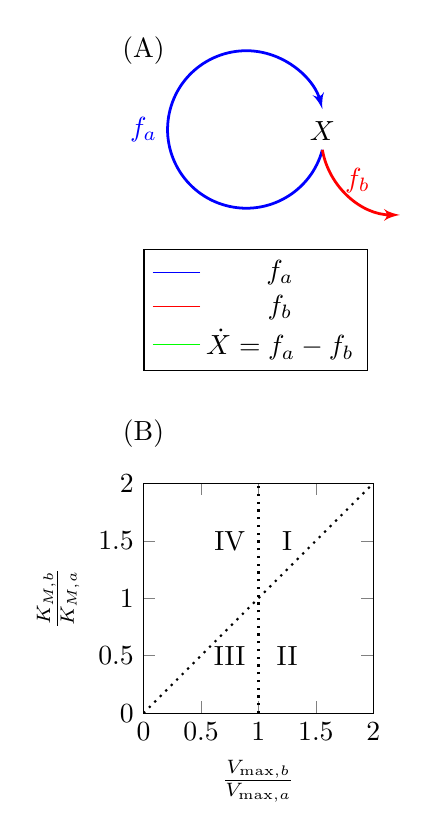
\begin{tikzpicture}[>=latex',node distance = 2cm]
            \node (X) {$X$};
            \draw [->,line width=1pt,blue] (X.south) arc (345:15:1cm) node [pos=0.5,left] (fa) {$f_a$};
            \draw [->,line width=1pt,red] (X.south) arc (190:270:1cm) node [pos=0.3,right] {$f_b$};
            \node [above of=fa,yshift=-1cm] (A) {(A)};
            \begin{customlegend}[legend entries={$f_a$,$f_b$,$\dot{X}=f_a-f_b$},legend style={below=2cm of fa,anchor=west,name=legend1}]
              \addlegendimage{blue,fill=black!50!red,sharp plot}
              \addlegendimage{red,fill=black!50!red,sharp plot}
              \addlegendimage{green,fill=black!50!red,sharp plot}
            \end{customlegend}
            \begin{axis}[name=phase,xmin=0,ymin=0,xmax=2,ymax=2,xlabel={$\frac{V_{\max,b}}{V_{\max,a}}$},ylabel={$\frac{K_{M,b}}{K_{M,a}}$},samples=6,at=(legend1.south west),anchor=above north west,width=4.5cm,height=4.5cm,yshift=-1.2cm]
            \addplot[domain=0:4,dotted,black,thick] {x};
            \addplot[dotted,black,thick] coordinates {(1,0) (1,2)};
            \node (one) at (axis cs:1.25,1.5) {I};
            \node (two) at (axis cs:1.25,0.5) {II};
            \node (three) at (axis cs:0.75,0.5) {III};
            \node (four) at (axis cs:0.75,1.5)(axis cs:1.25,0.5) {IV};
          \end{axis}
          \node [at=(legend1.south west),yshift=-0.8cm] (B) {(B)};
         \end{tikzpicture}}%
       \end{minipage}
       \hfill
       \begin{minipage}[c]{.65\linewidth}
        {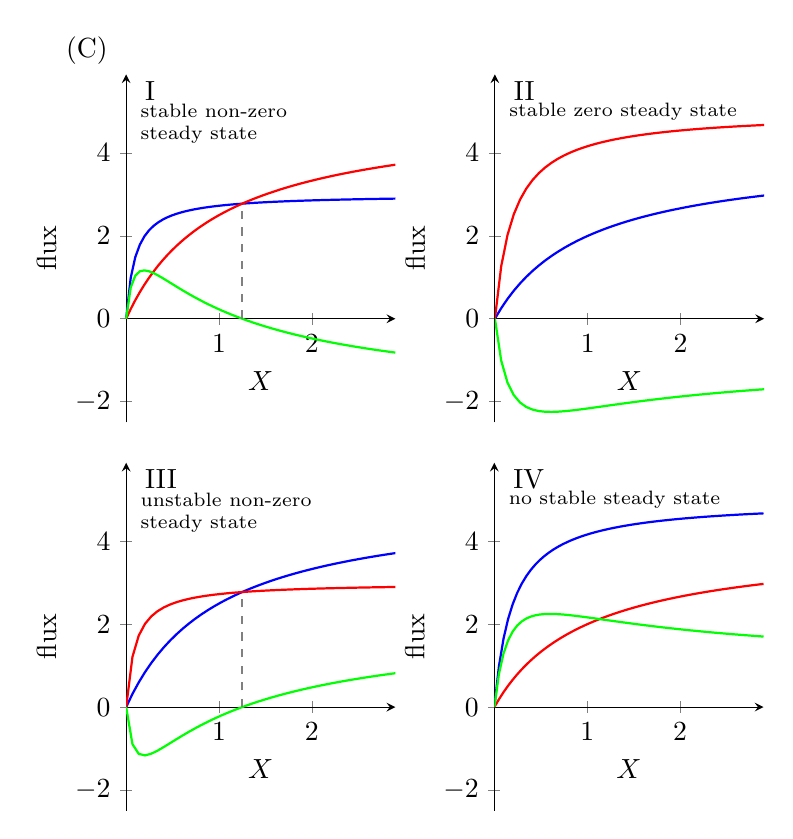
\begin{tikzpicture}
            \begin{axis}[name=plot1,axis x line=middle,axis y line=left,xlabel near ticks,ylabel near ticks,xmin=0,ymin=-2.5,xmax=2.9,ymax=5.9,xlabel={$X$},ylabel={flux},samples=60,width=5cm,height=6cm,clip=false]
            \addplot[domain=0:2.9,blue,thick] {3*x/(0.1+x)};
            \addplot[domain=0:2.9,red,thick] {5*x/(1+x)};
            \addplot[domain=0:2.9,green,thick] {3*x/(0.1+x)-5*x/(1+x)};
            \addplot[dashed,gray,thick] coordinates {(1.25,0) (1.25,2.77)};
            \node[right] (one) at (axis cs:0.1,5.5) {I};
            \node[right,align=left] (onetext) at (axis cs:0.05,4.7) {\scriptsize stable non-zero\\[-0.4em]\scriptsize steady state};
          \end{axis}
          \node [at=(plot1.north west),xshift=-0.5cm,yshift=0.3cm] (C) {(C)};

          \begin{axis}[name=plot2,axis x line=middle,axis y line=left,xlabel near ticks,ylabel near ticks,xmin=0,ymin=-2.5,xmax=2.9,ymax=5.9,xlabel={$X$},ylabel={flux},samples=60,at=(plot1.right of south east),anchor=left of south west,width=5cm,height=6cm]
            \addplot[domain=0:4,blue,thick] {4*x/(1+x)};
            \addplot[domain=0:4,red,thick] {5*x/(0.2+x)};
            \addplot[domain=0:4,green,thick] {4*x/(1+x)-5*x/(0.2+x)};
            \node[right] (two) at (axis cs:0.1,5.5) {II};
            \node[right,align=left] (twotext) at (axis cs:0.05,5) {\scriptsize stable zero steady state};
          \end{axis}

          \begin{axis}[name=plot3,axis x line=middle,axis y line=left,xlabel near ticks,ylabel near ticks,xmin=0,ymin=-2.5,xmax=2.9,ymax=5.9,xlabel={$X$},ylabel={flux},samples=60,at=(plot1.below south west),anchor=above north west,width=5cm,height=6cm,yshift=-0.5cm]
            \addplot[domain=0:4,blue,thick] {5*x/(1+x)};
            \addplot[domain=0:4,red,thick] {3*x/(0.1+x)};
            \addplot[domain=0:4,green,thick] {5*x/(1+x)-3*x/(0.1+x)};
            \addplot[dashed,gray,thick] coordinates {(1.25,0) (1.25,2.77)};
            \node[right] (three) at (axis cs:0.1,5.5) {III};
            \node[right,align=left] (threetext) at (axis cs:0.05,4.7) {\scriptsize unstable non-zero\\[-0.4em]\scriptsize steady state};
          \end{axis}

          \begin{axis}[name=plot4,axis x line=middle,axis y line=left,xlabel near ticks,ylabel near ticks,xmin=0,ymin=-2.5,xmax=2.9,ymax=5.9,xlabel={$X$},ylabel={flux},samples=60,at=(plot3.right of south east),anchor=left of south west,width=5cm,height=6cm]
            \addplot[domain=0:2.9,blue,thick] {5*x/(0.2+x)};
            \addplot[domain=0:2.9,red,thick] {4*x/(1+x)};
            \addplot[domain=0:2.9,green,thick] {5*x/(0.2+x)-4*x/(1+x)};
            \node[right] (four) at (axis cs:0.1,5.5) {IV};
            \node[right,align=left] (fourtext) at (axis cs:0.05,5) {\scriptsize  no stable steady state};
         \end{axis}
        \end{tikzpicture}}
       \end{minipage}
      \caption{\label{fig:simplecycle}
        (A) A simple auto-catalytic cycle induces two fluxes, $f_a$ and $f_b$ as a function of the concentration of $X$.
        These fluxes follow simple Michaelis Menten kinetics.
        A steady state occurs when $f_a=f_b$, implying that $\dot{X}=0$.
        The cycle always has a steady state at $X=0$.
        The slope of each reaction at $X=0$ is $V_{\max}/K_m$.
        A steady state is stable if at the steady state point $\frac{d\dot{X}}{dX}<0$.
        (B) Each set of kinetic parameters, $V_{\max,a},V_{\max,b},K_{M,a},K_{M,b}$ results in one of four cases (C): 
       (I) there is a stable positive steady state and zero is an unstable steady state; 
       (II) zero is the only non-negative steady state, and it is stable;
       (III) zero is a stable steady state and there is a positive, non-stable steady state; 
       (IV) zero is the only non-negative steady state and it is unstable.}
    \end{figure}

    We characterize the metabolic state of this system by the concentration of the metabolite $X$.
    We note that knowing the concentration of $X$ suffices in order to calculate the fluxes originating from it, $f_a$ and $f_b$, thus fully defining the state of the system.
    A steady state of the system is defined as a concentration, $X^*$, which induces fluxes that keep the concentration steady, such that the total in-flux to $X$ is exactly equal to the total out-flux from it.
    In our example, the outgoing flux from $X$ is $f_a+f_b$ and the incoming flux to $X$ is $2f_a$, so at steady state it holds that:
    \begin{equation}
      \label{eq:xdyna}
      \dot X = \frac{dX}{dt} = 2f_a - (f_a + f_b) = 0
    \end{equation}

    Expanding this condition we get:
    \begin{equation*}
      \dot X = 0 \Rightarrow f_a = f_b \Rightarrow \frac{V_{\max,a}X}{K_{M,a}+X}=\frac{V_{\max,b}X}{K_{M,b}+X}
    \end{equation*}
    which is satisfied either if $X=0$ or if:
    \begin{equation}
      \label{eq:xstst}
      X=\frac{V_{\max,b}K_{M,a}-V_{\max,a}K_{M,b}}{V_{\max,a}-V_{\max,b}}
    \end{equation}
    As physiologically the concentration of $X$ cannot be negative, we get a constraint on the kinetic parameters for which a positive steady state exists:
    \begin{equation*}
      \frac{V_{\max,b}K_{M,a}-V_{\max,a}K_{M,b}}{V_{\max,a}-V_{\max,b}}>0 \Rightarrow \frac{\frac{V_{\max,b}}{K_{M,b}}-\frac{V_{\max,a}}{K_{M,a}}}{V_{\max,a}-V_{\max,b}}>0
    \end{equation*}
    The constraint states that if $V_{\max,a}>V_{\max,b}$ then it must be that $\frac{V_{\max,b}}{K_{M,b}}>\frac{V_{\max,a}}{K_{M,a}}$ and that if $V_{\max,a}<V_{\max,b}$ then $\frac{V_{\max,b}}{K_{M,b}}<\frac{V_{\max,a}}{K_{M,a}}$.
    As $\frac{V_{\max}}{K_m}$ is the slope of the Michaelis Menten function at $X=0$, the constraint implies that in order for a positive steady state to exist, the reaction with higher maximal flux must have a shallower slope at $X=0$.
    This condition can be intuitively understood as the reaction with shallower slope at $X=0$ has smaller fluxes for small values of $X$, compared with the other reaction, so unless it has higher fluxes than the other reaction for large values of $X$ (meaning that its maximal flux is higher), the two will not intersect.
    This constraint is graphically illustrated in Figure \ref{fig:simplecycle}B where cases (II) and (IV) have no positive steady states, and cases (I) and (III) have a positive steady state.

    While having a positive concentration steady state is an essential condition to sustain flux, it is not sufficient.
    The positive concentration steady state must also be stable to small perturbations.
    Stability with respect to small perturbations is determined by the response of the system to small deviations from the steady state, $X^*$.
    Mathematically, stability dictates that at $X=X^*$ it holds that $\frac{d\dot X}{dX} <0$, as this  implies that for points with a small deviation from the steady state: $X = X^*+\Delta X$ the net flux $\dot X$ will oppose the direction of the deviation.
    If $\Delta X$ is positive then $\dot X$ will be negative at $X^*+\Delta X$, reducing $X$ back to $X^*$, and if $\Delta X$ is negative, $\dot X$ will be positive, increasing $X$ back to $X^*$.

    For the simple kinetics we chose the stability condition requires that:
    \begin{equation*}
      \frac{d\dot X}{dX}\Big\vert_{X^*} = \frac{V_{\max,a}K_{M,a}}{(K_{M,a}+X^*)^2}-\frac{V_{\max,b}K_{M,b}}{(K_{M,b}+X^*)^2}<0
    \end{equation*}
    Substituting for $X^*=0$ gives that $0$ is a stable steady state point if $\frac{V_{\max,a}}{K_{M,a}}<\frac{V_{\max,b}}{K_{M,b}}$ (corresponding to the area below the diagonal in figure \ref{fig:simplecycle}B, where $\frac{V_{\max,b}}{V_{\max,a}}>\frac{K_{M,b}}{K_{M,a}}$ resulting in cases (II) and (III)) and is unstable otherwise.
    For  the non-zero steady state, $X^*=\frac{V_{\max,b}K_{M,a}-V_{\max,a}K_{M,b}}{V_{\max,a}-V_{\max,b}}$, we get the opposite condition, i.e. that it is stable if $\frac{V_{\max,b}}{V_{\max,a}}<\frac{K_{M,b}}{K_{M,a}}$ and unstable otherwise.

    It is worthwhile noting that the stability criteria can be stated in metabolic control terms \cite{Fell1997} as requiring that the elasticity of the biomass reaction at the positive steady state be greater than the elasticity of the autocatalytic reaction:
    \begin{equation*}
      \frac{df_b}{dX}\Big\vert_{X^*}>\frac{df_a}{dX}\Big\vert_{X^*} \Rightarrow \epsilon^X_b>\epsilon^X_a
    \end{equation*}
    
    The complete analysis is summed up in Figure \ref{fig:simplecycle}B.
    Domains (I) and (III) represent cases where a positive steady state point exists.
    The domains below the diagonal represent cases where $X^*=0$ is a stable steady state point, and the other steady state, if it exists is unstable (cases (II) and (III)).
    The domains above the diagonal represent cases where $X^*=0$ is an unstable steady state point, and the other steady state, if it exists is stable (cases (I) and (IV)).

    To conclude, for this simple cycle, we get that in order for a positive-concentration stable steady state to exist, two conditions must be satisfied:
    \begin{equation}
    \label{eq:stabconds}
    \begin{dcases}
      & V_{\max,b}>V_{\max,a} \\
      & \frac{V_{\max,a}}{K_{M,a}}>\frac{V_{\max,b}}{K_{M,b}}
    \end{dcases}
    \end{equation}
    meaning that for high enough a concentration of $X$, the biomass generating flux should be higher than the auto-catalytic flux, ensuring stability, and that at zero concentration of $X$, the slope of the auto-catalytic reaction is steeper than the slope of the biomass generating reaction, ensuring that the two fluxes will be equal for some positive concentration of $X$.

    Interestingly, these conditions imply that if $K_{M,b}<K_{M,a}$ then no positive stable steady state can be achieved, even when allowing changes to the expression levels of the enzymes catalyzing $f_a$ and $f_b$, which only affect $V_{\max,a}$ and $V_{\max,b}$.
    
\subsection{Input flux increases the range of parameters for which a stable steady state solution exists}
    Real auto-catalytic cycles are not stand-alone constructs and specifically, such cycles generally have some fueling reactions with input flux to at least some of their intermediate metabolites.
    When adding a constant input flux, $f_i$ to our simple system (Figure \ref{fig:inputcycle}A) the steady state condition changes to include this flux, giving:
    \begin{equation*}
      \dot X = \frac{dX}{dt} = f_i + f_a - f_b = 0
    \end{equation*}
    In this model, at $X=0$, $\dot X=f_i>0$ so the concentration of $X$ increases and there is no steady state at zero.
    If $V_{\max,b}>f_i+V_{\max,a}$ then at large enough value of $X$, $\dot X$ will be negative, implying that at some value of $X$ between these two extremes $\dot{X}$ attains the value of zero, such that under this condition a positive stable steady state point exists (Figure \ref{fig:inputcycle} (I)).
    This case therefore differs from the case with no input flux analyzed above, as now a positive stable steady state can always be achieved by modifying only $V_{\max,a}$ and/or $V_{\max,b}$.
    In this setup cells can therefore tune the expression levels of enzymes to meet the needs of a stable steady state flux.

    In cases where $V_{\max,b}<f_i+V_{\max,a}$ either no steady states exist (Figure \ref{fig:inputcycle} (II)), or two positive steady states exist (Figure \ref{fig:inputcycle} (III)).
    The latter case implies that there exists a positive concentration $X$ that satisfies:
    \begin{equation*}
        \dot X = 0 \Rightarrow f_i + f_a(X) - f_b(X) = 0 \Rightarrow f_i+\frac{V_{\max,a}X}{K_{M,a}+X} = \frac{V_{\max,b}X}{K_{M,b}+X}
    \end{equation*}
  In this case, the lower concentration steady state will be stable.
    \begin{figure}[h!]
      \centering
      \begin{minipage}[c]{0.8\linewidth}%
        {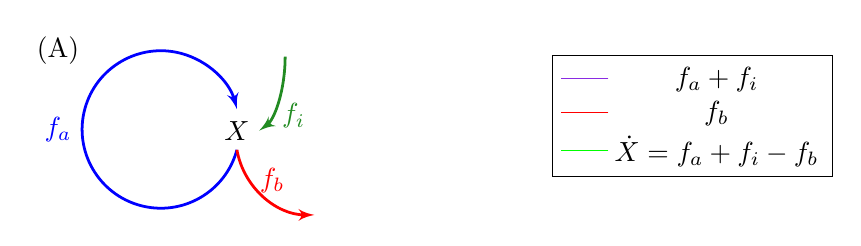
\begin{tikzpicture}[>=latex',node distance = 2cm]
            \node (X) {$X$};
            \draw [->,line width=1pt,blue] (X.south) arc (345:15:1cm) node [pos=0.5,left] (fa) {$f_a$};
            \draw [->,line width=1pt,red] (X.south) arc (190:270:1cm) node [pos=0.3,right] {$f_b$};
            \draw [<-,line width=1pt,ForestGreen] (X.east) arc (-70:0:0.5cm and 1cm) node [pos=0.3,right] (fi) {$f_i$};
            \node [above of=fa,yshift=-1cm] (A) {(A)};
            \begin{customlegend}[legend entries={$f_a+f_i$,$f_b$,$\dot{X}=f_a+f_i-f_b$},legend style={right=3cm of fi,anchor=west,name=legend1}]
              \addlegendimage{BlueViolet,fill=black!50!red,sharp plot}
              \addlegendimage{red,fill=black!50!red,sharp plot}
              \addlegendimage{green,fill=black!50!red,sharp plot}
            \end{customlegend}
         \end{tikzpicture}}%
       \end{minipage}

       \begin{minipage}[c]{\linewidth}%
        {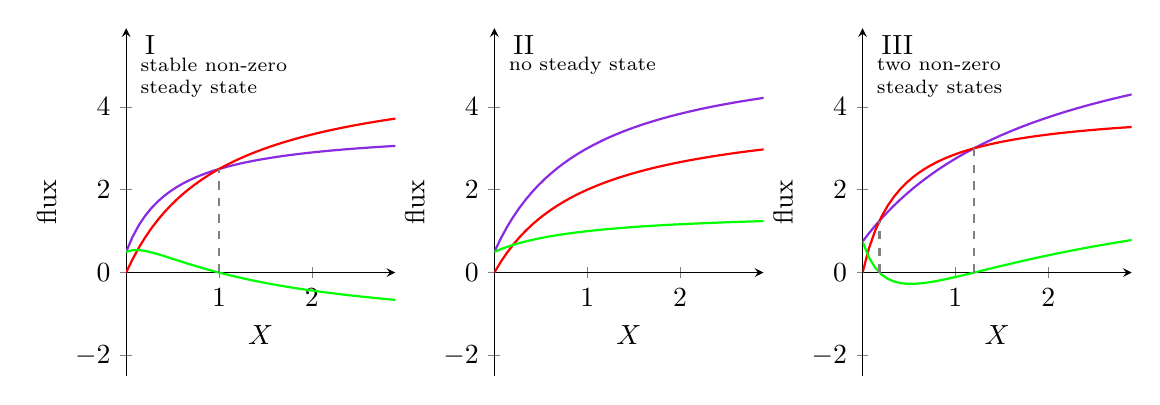
\begin{tikzpicture}
            \begin{axis}[name=plot1,axis x line=middle,axis y line=left,xlabel near ticks,ylabel near ticks,xmin=0,ymin=-2.5,xmax=2.9,ymax=5.9,xlabel={$X$},ylabel={flux},samples=60,width=5cm,height=6cm]
            \addplot[domain=0:4,BlueViolet,thick] {3*x/(0.5+x)+\influx};
            \addplot[domain=0:4,red,thick] {5*x/(1+x)};
            \addplot[domain=0:4,green,thick] {3*x/(0.5+x)-5*x/(1+x)+\influx};
            \addplot[dashed,gray,thick] coordinates {(1,0) (1,2.5)};
            \node[right] (one) at (axis cs:0.1,5.5) {I};
            \node[right,align=left] (onetext) at (axis cs:0.05,4.7) {\scriptsize stable non-zero\\[-0.4em]\scriptsize steady state};
          \end{axis}

          \begin{axis}[name=plot2,axis x line=middle,axis y line=left,xlabel near ticks,ylabel near ticks,xmin=0,ymin=-2.5,xmax=2.9,ymax=5.9,xlabel={$X$},ylabel={flux},samples=60,at=(plot1.right of south east),anchor=left of south west,width=5cm,height=6cm]
            \addplot[domain=0:4,BlueViolet,thick] {5*x/(1+x)+\influx};
            \addplot[domain=0:4,red,thick] {4*x/(1+x)};
            \addplot[domain=0:4,green,thick] {5*x/(1+x)-4*x/(1+x)+\influx};
            \node[right] (two) at (axis cs:0.1,5.5) {II};
            \node[right,align=left] (twotext) at (axis cs:0.05,5) {\scriptsize no steady state};
          \end{axis}

          \begin{axis}[name=plot3,axis x line=middle,axis y line=left,xlabel near ticks,ylabel near ticks,xmin=0,ymin=-2.5,xmax=2.9,ymax=5.9,xlabel={$X$},ylabel={flux},samples=60,at=(plot2.right of south east),anchor=left of south west,width=5cm,height=6cm]
            \addplot[domain=0:4,BlueViolet,thick] {6*x/(2+x)+1.5*\influx};
            \addplot[domain=0:4,red,thick] {4*x/(0.4+x)};
            \addplot[domain=0:4,green,thick] {6*x/(2+x)-4*x/(0.4+x)+1.5*\influx};
            \addplot[dashed,gray,thick] coordinates {(1.2,0) (1.2,3)};
            \addplot[dashed,gray,thick] coordinates {(0.182,0) (0.182,1.25)};
            \node[right] (three) at (axis cs:0.1,5.5) {III};
            \node[right,align=left] (threetext) at (axis cs:0.05,4.7) {\scriptsize two non-zero\\[-0.4em]\scriptsize steady states};
          \end{axis}
        \end{tikzpicture}}
       \end{minipage}
      \caption{\label{fig:inputcycle}
        (A) A simple auto-catalytic cycle with a fixed input flux, $f_i$.
        A steady state occurs when $f_a+f_i=f_b$.
        If $V_{\max,b}>V_{\max,a}+f_i$ then there is always a single stable steady state (I).
        If $V_{\max,b}<V_{\max,a}+f_i$ then there can either be no steady states (II), or two steady states where the smaller one is stable (III).
      }
    \end{figure}
    \subsection{Generalizing for different auto-catalytic stoichiometries}
    Our initial analysis considered an auto-catalytic reaction with $1:2$ stoichiometry, such that for every substrate molecule consumed, two were produced.
    Real-world auto-catalytic cycles may have different stoichiometries.
    For example, the CBB cycle has a stoichiometry of $5:6$ so that for every 5 molecules of 5-carbon sugars that the auto-catalytic reaction consumes, 6 5-carbon sugars are produced.
    We can generalize our analysis by defining $\alpha$ such that for every molecule of $X$ that $f_a$ consumes, it produces $1+\alpha$ molecules of $X$, where $\alpha$ may be a fraction.
    This extension implies that equation \eqref{eq:xdyna} becomes:

    \begin{equation*}
      \dot X = \frac{dX}{dt} = (1+\alpha)f_a - (f_a + f_b) = 0 \Rightarrow \alpha f_a = f_b \Rightarrow \frac{\alpha V_{\max,a}X}{K_{M,a}+X}=\frac{V_{\max,b}X}{K_{M,b}+X}
    \end{equation*}

    Therefore, all of the mathematical derivations conducted above can be repeated, replacing $V_{\max,a}$ by $\alpha V_{\max,a}$.

    The steady states of this system are thus $X=0$ and (from equation \eqref{eq:xstst}):
    \begin{equation*}
      X=\frac{V_{\max,b}K_{M,a}-\alpha V_{\max,a}K_{M,b}}{\alpha V_{\max,a}-V_{\max,b}}
    \end{equation*}

    The stability criteria from equation \eqref{eq:stabconds} become:
    \begin{equation*}
    \begin{dcases}
      & V_{\max,b}>\alpha V_{\max,a} \\
      & \frac{\alpha V_{\max,a}}{K_{M,a}}>\frac{V_{\max,b}}{K_{M,b}}
    \end{dcases}
    \end{equation*}
    So the qualitative conditions and observations from the $2:1$ stoichiometry case remain valid but with a constant factor that changes the quantitative relations according to the relevant stoichiometry.

\section{Discussion}
A common concept in synthetic biology is that the successful implementation of novel pathways requires the expression of functional enzymes in the correct amounts in a target organizm.
Here we show that in the specific context of the newly introduced enzymes being involved in auto-catalytic cycles, such a successful expression may not suffice.
Specifically, changes to some of the kinetic parametars of the enzymes may be required in order for the novel pathway to function.

Another aspect of our findings is that while generally, increased affinity and catalytic rate are economically beneficial for enzymes, in the specific context of auto-catalytic cycles constraints may exist on the relations between these kinetic parameters across different enzymes rendering improvements in only some of them destructive for the functioning of the cycle.

A recent example of these two conclusions in vivo is the implementation of a functional CBB cycle in \emph{e.coli} by introducing the two genes missing for its functioning.
The successful introduction of the genes did not suffice to make the cycle functioning and further directed evolution was needed in order to achieve non-zero flux.
A key change in the evolution was the decrease of the affinity of PRS, the enzyme responsible for the flux out of the CBB cycle, corresponding to the biomass reaction in our simple model.
\section{Acknowledgments}
We would like to thank Elad Noor, Arren Bar-Even, Dan Davidi, Yinon Bar-On, Katja Tummler, Daniel Segre, Niv Antonovsky, Matthias Heinemann and \dots for fruitful discussions and valuable insights contributing to this work.
\bibliography{library}{}
\bibliographystyle{ieeetr}
\end{document}
